\documentclass[11pt, oneside]{article} 
\usepackage{geometry}
\geometry{letterpaper} 
\usepackage{graphicx}
	
\usepackage{amssymb}
\usepackage{amsmath}
\usepackage{parskip}
\usepackage{color}
\usepackage{hyperref}

\graphicspath{{/Users/telliott/Dropbox/Github-Math/quickgeo/figures/}{/Users/telliott/Dropbox/Github-Math/figures/}}
% \begin{center} \includegraphics [scale=0.4] {gauss3.png} \end{center}

\title{Isosceles triangles}
\date{}

\begin{document}
\maketitle
\Large

%[my-super-duper-separator]

We continue in this chapter with the subject of congruence and our second major theorem.  The first one was the triangle sum theorem.  In this chapter we will prove the isosceles triangle theorem.  

$\bullet$  \ Given that two sides are equal in a triangle (it is isosceles), the base angles opposite those sides are also equal.

\begin{center} 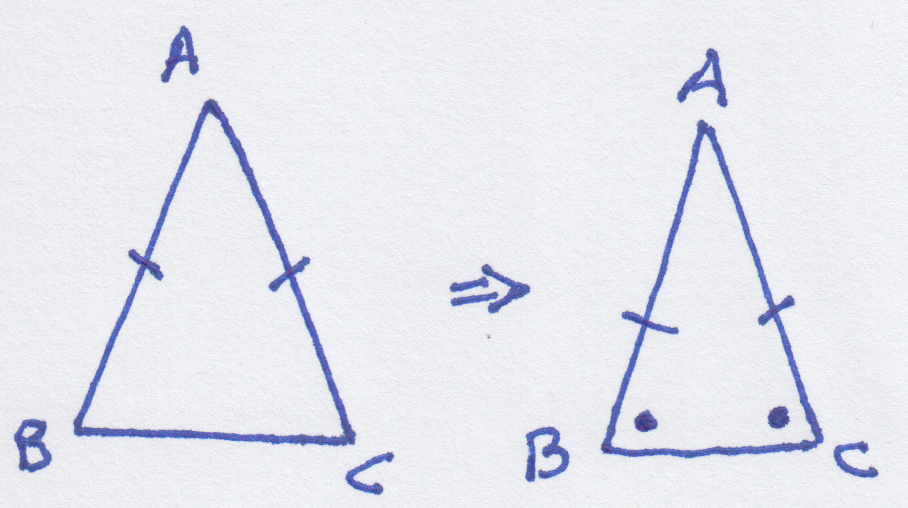
\includegraphics [scale=0.25] {C9.png} \end{center}
We're given that $AB = AC$.  We claim that $\angle B = \angle C$.

I think we can agree, to begin with, that this seems rather obvious.  After all, what reason would you give for saying that the two angles are different?  Perhaps you are right-handed and have a bias toward the right angle being larger.

But then, imagine looking at a reflection of the triangle.  We said that reflection is legal.  Now right has become left, and the angle on the left side is the larger one.  That makes no sense.

\emph{Proof}.

A simple proof is to draw the angle bisector of the angle at $A$, the line that splits the angle in half.  We'll give a method for doing that later.
\begin{center} 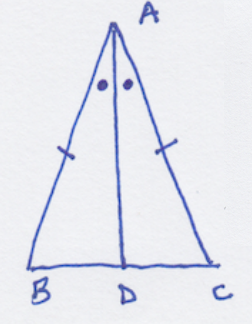
\includegraphics [scale=0.4] {C8b.png} \end{center}

Since $AB = AC$, and side $AD$ is shared, we have two pairs of equal sides.  The angle bisector construction makes $\angle BAD = \angle DAC$ at the top vertex.  

Therefore, the two smaller triangles are congruent, by SAS.

Since $\triangle ADB \cong \triangle ACD$, it follows that the angles at $B$ and $C$ are equal.

It also follows that the base is cut into two equal pieces ($BD = DC$), and that the two angles at $D$ are equal, which makes them both right angles.

$\square$

\subsection*{converse of isosceles triangle theorem}

The converse of the isosceles triangle theorem is also true.

The forward version is that if two sides are equal in a triangle, then the sides opposite are equal.  The converse is that if two angles are equal in a triangle, then the sides opposite are equal.

It isn't alway the case that the converse of a true theorem is true.  We must prove (or at least try to prove) each case.

$\bullet$  \ Given two equal sides at the base of a triangle, the sides are also equal and the triangle is isosceles.

\emph{Proof}.

Draw the angle bisector again.  Now, we have two smaller triangles with two angles equal, since we are given that the base angles are equal.
\begin{center} 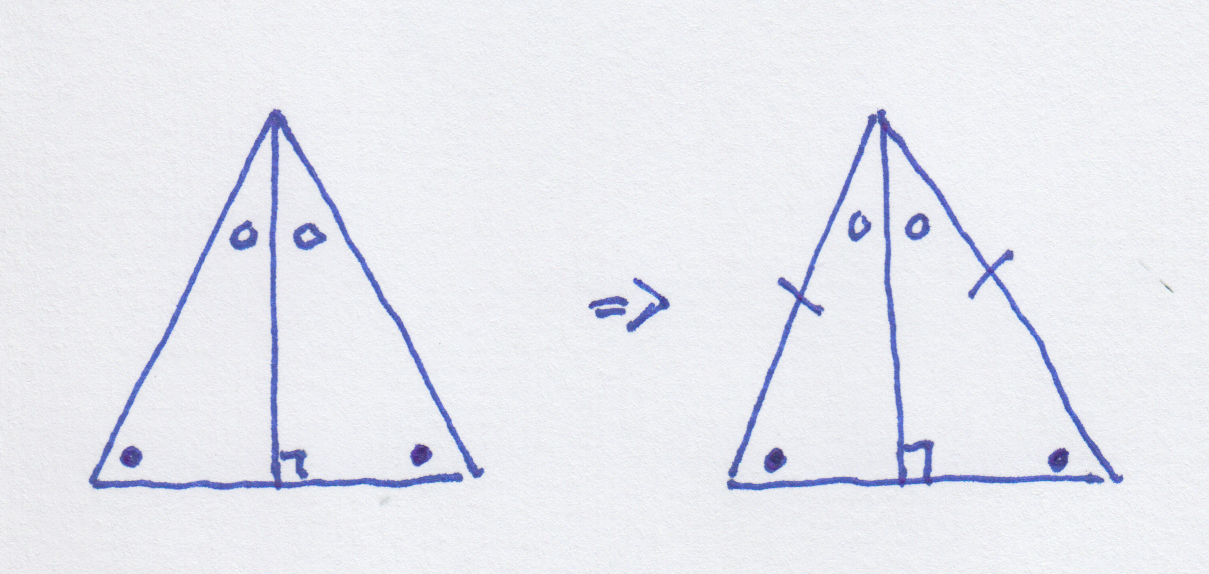
\includegraphics [scale=1.0] {C10.png} \end{center}

In comparing these two smaller triangles, the third angle must also be equal, by the triangle sum theorem.  This is the angle where the bisector meets the base.  Since the pair of them are equal and also supplementary, they are both right angles. 

Then the shared side between the right angle and the one at the top marked with the open circle, gives ASA and therefore, the two smaller triangles are congruent.

It follows that the two sides of the original triangle are equal.

$\square$

\subsection*{Euclid's proof}

Let's approach the same problem a different way.  We're going to look at two different triangles inside the same figure.
\begin{center} 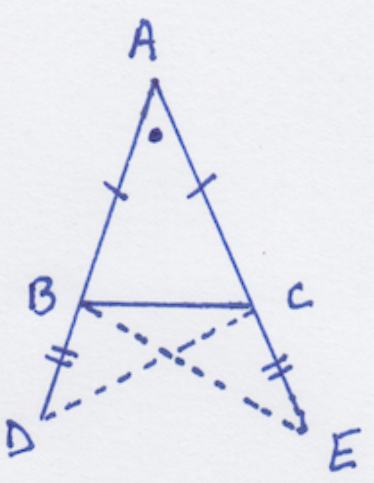
\includegraphics [scale=0.3] {C3.png} \end{center}
In the diagram above we have two sides of $\triangle ABC$ that have been extended as far as $D$ and $E$.  We know (we're \emph{given}) that $AB = AC$ and $AD = AE$, and by subtraction of equals, we know that $BD = CE$.

The apex $\angle A$ is, of course, equal to itself, so it's marked with a dot as a reminder.

Now, look at the two triangles that have one side as a dotted line.  I mean $\triangle ACD$ and $\triangle ABE$.  
\begin{center} 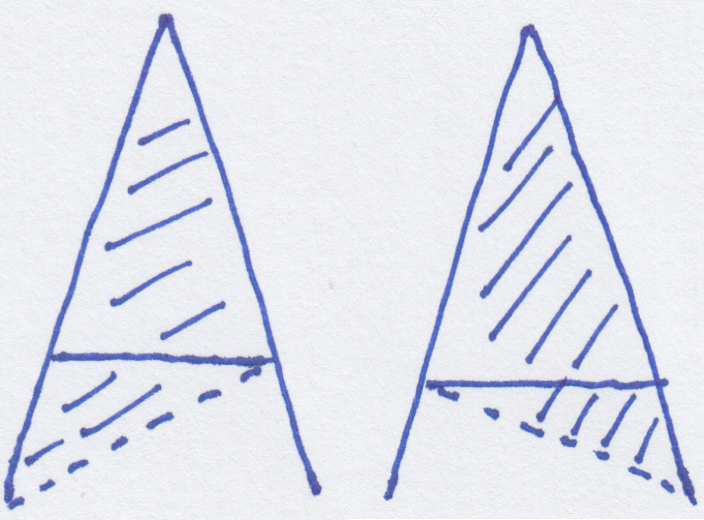
\includegraphics [scale=0.25] {C3a.png} \end{center}
It's a little tricky because they overlap each other and are also mirror images.  Be sure you trace out the correct three vertices for each one.

We were given

$\circ$ \ $AB = AC$

$\circ$ \ $AD = AE$

$\circ$ \ $\angle A$ is certainly equal to itself.

By subtraction: 

$\circ$ \ $BD = CE$

$\circ$ \ $BC$ is certainly equal to itself

Since $\angle A$ is shared (it's exactly the same in both triangles), we have SAS.  We conclude that the two $\triangle$ are congruent:  $\triangle ACD \cong \triangle ABE$.

\begin{center} 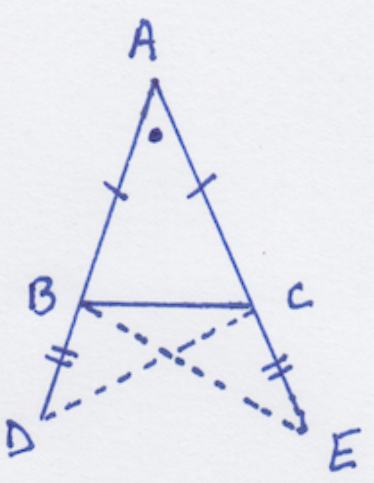
\includegraphics [scale=0.3] {C3.png} \end{center}

Now that we know they are congruent, it follows that there are other equalities:

$\circ$ \ $BE = CD$

$\circ$ \ $\angle D = \angle E$

$\circ$ \ $\angle ABE = \angle ACD$

I have marked the first pair with larger dots because what we have shown so far is only that two angles, taken together, are equal.  We must still find a way that the individual components are equal.

In the second step we will show that the angles marked with magenta dots are equal (below).  Then subtraction will give the result we are after, that the red dotted angles are equal.

\begin{center} 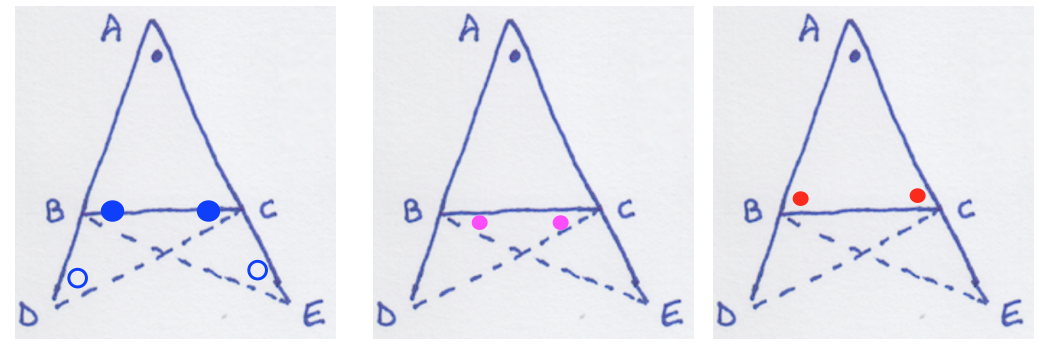
\includegraphics [scale=0.35] {C3b.png} \end{center}

Again,  the goal is to show that $\angle ABC = \angle ACB$.  We already have equal angles that include those two, namely $\angle ABE = \angle ACD$.  Now we need to show that $\angle CBE = \angle BCD$ (magenta dots).

We will show that $\triangle BCD \cong \triangle BCE$.  We have that the sides flanking $\angle D$ and $\angle E$ are equal.  Check above to see which statements apply.  We also have that $\angle D =\angle E$.

We conclude that $\triangle BCD \cong \triangle BCE$ by SAS.  

Therefore, by congruent triangles, $\angle CBE = \angle BCD$.

And finally, since  $\angle ABE = \angle ACD$ (left panel) and $\angle CBE = \angle BCD$ (middle panel), subtract the second from the first to obtain the base angles.
\[ \angle ABC = \angle ACB \]

$\square$

This is a moderately complicated proof of the isosceles triangle theorem.  It's more challenging than the first one, but Euclid proves it before dealing with angle bisection, so he can't use that idea here.

Euclid also proves the converse.  He uses a method that we haven't seen yet, so let's not worry about it for now.

Historically the diagram is known as the "bridge of asses" (\emph{pons asinorum} in Latin), because it looks something like a bridge, and asses (that is, dullards), proved incapable of being led over it.

\begin{center} 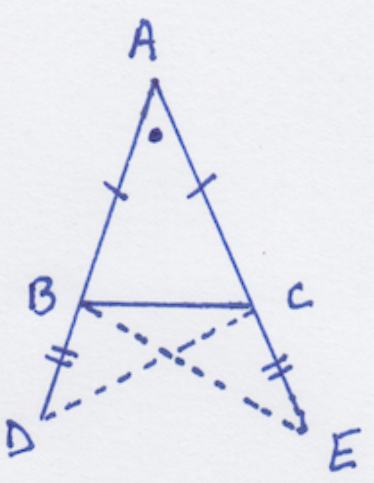
\includegraphics [scale=0.3] {C3.png} \end{center}

\subsection*{SSS $\rightarrow$ SAS}

Continuing with a theorem from the last chapter, a third method for proving congruence is SSS.

\emph{Proof}.

Suppose that $\triangle ABC$ and $\triangle ABD$ have all three sides equal.  Then place the two triangles together to form a kite, two pairs of adjacent sides equal, and one side shared.
\begin{center} \includegraphics [scale=0.6] {SSSb.png} \end{center}

Draw $CD$.  By the forward version of the isosceles triangle theorem, the angles marked with open dots are equal, as are the angles marked with filled dots.  Therefore $\angle D = \angle C$.  

We have SAS, so $\triangle ABC \cong \triangle ABD$.

$\square$


\end{document}
